Программное обеспечение для считывания, обработки и хранения информации с подсистем детектора, в эксперименте Belle II объединено вместе с медленным контролем, в систему сбора данных (DAQ). Задачей данной системы является считывание сигналов детектора по решению триггера первого уровня (L1). Система передает данные с электроники через несколько модулей, предназначенных для обработки данных, затем данные помещаются в систему хранения. Основными модулями обработки данных являются\cite{TechRep}:
\begin{itemize}
  \item Канал передачи данных Belle2Link. Данный канал представляет собой высокоскоростное оптическое волокно с пропускной способностью 3.125 Гб/с
  \item Универсальная платформа считывания данных COPPER. Каждый модуль COPPER представляет собой компьютер с ОС Linux и процессором Intel Atom работающем на частоте 1.6 ГГц. Скорость обработки данных одного модуля составляет $10^6$ слов/с. В DAQ размещено несколько сотен модулей COPPER
%  \item Система построения событий?
  \item Считывающий компьютер. Данный компьютер представляет собой сервер, который  работает на двух процессорах Intel Core i7, работающих на частоте 3.3 ГГц. Скорость обработки данных каждого компьютера составляет $1.6\cdot10^7$ слов/с. Порядка 50 таких компьютеров подключено к COPPER
  \item Система высокоуровневых триггеров (HLT). HLT состоит из нескольких блоков кластеров ПК, в которых один кластер состоит из 20 серверов ПК с двумя процессорами Core i7. С 10 единицами кластеров ПК общее количество ядер оценивается в 1600 со скоростью обработки данных $0.5\cdot10^6$ слов/с на ядро.
\end{itemize}
На рисунке 7 показан глобальный дизайн системы Belle II DAQ. 
\begin{figure}[htp]
  \centering
  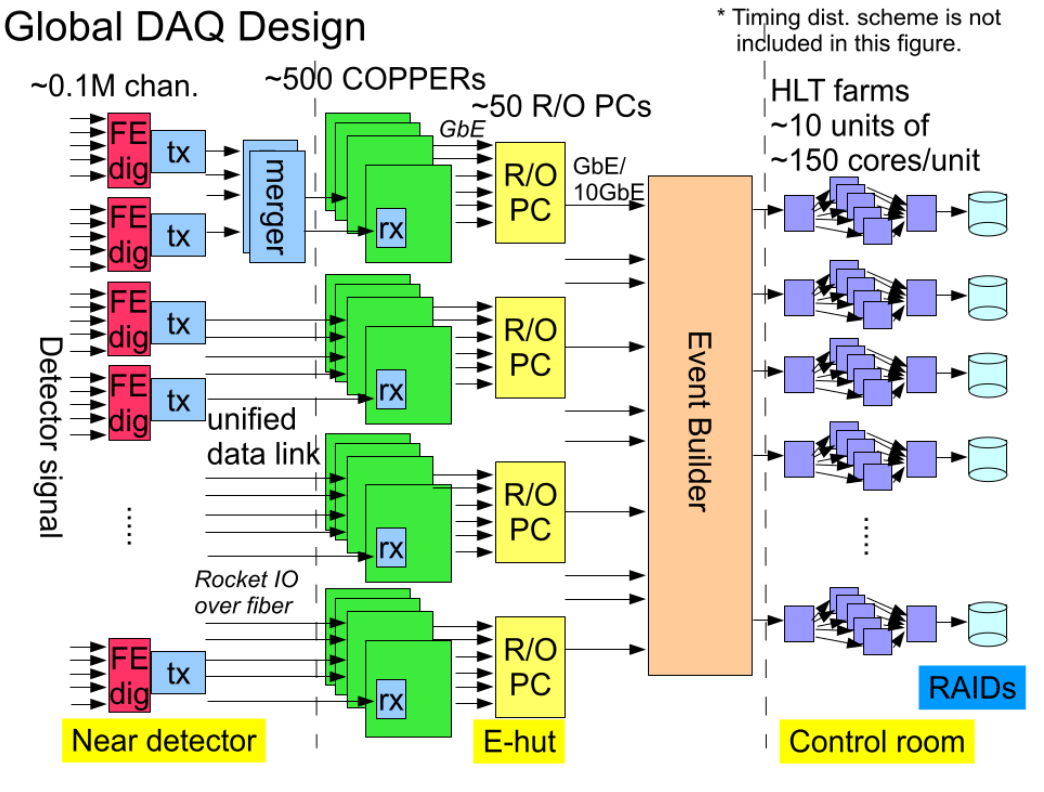
\includegraphics[width=0.9\textwidth]{daq}
  \caption{Схема устройства системы сбора данных DAQ.}
  \label{fig:galaxy}
\end{figure}
Данные, пришедшие с различных подсистем детектора, оцифровываются в считывающей электронике (FEE), затем оцифрованные сигналы передаются в системы COPPER по длинным оптическим волокнам по каналу передачи данных Belle2Link. Дальнейшее построение событий происходит на компьютерах системы сбора данных, которые получили данные через Ethernet. Затем данные передаются в фермы HLT для последующего отбора программных событий. После прохождения фермы HLT, данные помещаются в ячейки хранилища. Ячейка представляет собой RAID массив, который  имеет 4 набора по 12 дисков объемом 3 Тб каждый\cite{DAQ}.\par
  Сложной задачей при проектировании системы сбора данных являлось то, что при такой проектной светимости события поступают с частотой 20 кГц, следовательно, необходимо было разработать систему, способную обрабатывать входные данные с частотой 30 кГц. Объем входных сырых данных составляет порядка 1 Мб.
